\documentclass{article}
\usepackage[left=2cm, right=2cm, top=2cm, bottom=4.0cm]{geometry}
\usepackage[utf8]{inputenc}
\usepackage[english]{babel}
\usepackage{natbib}
\usepackage{float}
\usepackage[version=4]{mhchem}
\usepackage{graphicx}
\usepackage{fancyhdr}
\usepackage{amssymb}
\usepackage{mathtools}
\usepackage{gensymb}
\usepackage{lastpage}
\pagestyle{fancy}
\usepackage{pdfpages}
\usepackage{xcolor}
\usepackage{listings}
\usepackage{minted}
\usepackage{amsmath}
\lstloadlanguages{csh}
\usepackage{subfigure} 
\lstdefinestyle{sharpc}{language=[Sharp]C, frame=lr, rulecolor=\color{blue!80!black}}

\lstset{ 
  language=R,                     % the language of the code
  basicstyle=\tiny\ttfamily, % the size of the fonts that are used for the code
  numbers=left,                   % where to put the line-numbers
  numberstyle=\tiny\color{Blue},  % the style that is used for the line-numbers
  stepnumber=1,                   % the step between two line-numbers. If it is 1, each line
                                  % will be numbered
  numbersep=5pt,                  % how far the line-numbers are from the code
  backgroundcolor=\color{white},  % choose the background color. You must add \usepackage{color}
  showspaces=false,               % show spaces adding particular underscores
  showstringspaces=false,         % underline spaces within strings
  showtabs=false,                 % show tabs within strings adding particular underscores
  frame=single,                   % adds a frame around the code
  rulecolor=\color{black},        % if not set, the frame-color may be changed on line-breaks within not-black text (e.g. commens (green here))
  tabsize=2,                      % sets default tabsize to 2 spaces
  captionpos=b,                   % sets the caption-position to bottom
  breaklines=true,                % sets automatic line breaking
  breakatwhitespace=false,        % sets if automatic breaks should only happen at whitespace
  keywordstyle=\color{blue},      % keyword style
  commentstyle=\color{green},   % comment style
  stringstyle=\color{black}      % string literal style
} 

\fancyhf{}
\newenvironment{normaltext}[1][]%
  {#1}%
  {}
%\chead{Page \thepage \hspace{1pt} of \pageref{LastPage}}
\chead{Page \thepage \hspace{1pt} of 17}
\newcommand{\todo}[1]{\textcolor{red}{TODO: #1} \PackageWarning{TODO:}{#1}}
\fancypagestyle{firstpage}{
  \hoffset = -10pt
  \headheight = 23pt
  \headsep = 10pt
  \topmargin = 0em
  \textheight = 0pt
  \footskip = 20.5pt
  \chead{}
  \renewcommand{\headrulewidth}{0pt}
  \lhead{PE Physik Engines \\FS24}
  \rhead{Aufgabe 3\\}
  \lfoot{Zürich, 29. Mai 2023}
  \rfoot{
  \begin{tabular}{p{5cm}|p{5cm}}  \\ 
        \hrulefill & \hrulefill \\
        Dario Brunner & Timo Sigrist 
        \end{tabular}
}
  \cfoot{\vspace*{5\baselineskip}}
  }
  \fancypagestyle{app}{
  \hoffset = -10pt
  \headheight = 23pt
  \headsep = 10pt
  \topmargin = 0em
  \textheight = 0pt
  \footskip = 20.5pt
  \chead{}
  \renewcommand{\headrulewidth}{0pt}
  \lhead{}
  \rhead{}
  \lfoot{}
  \rfoot{}
  \cfoot{\vspace*{5\baselineskip}}
  }


\begin{document}

\begin{titlepage}
\thispagestyle{empty} % Remove page numbers and headers/footers
     \vspace*{6em}{\centering\huge\textbf{Semesterprojekt Modul PE FS 2024} \par}
     
     \vspace*{5em}
     \raggedright % Align to the left
     \textbf{Authoren}\\
     \vspace*{1em}
     Dario Brunner,\\
     ZHAW Student School of Engineering, Computer Science BSc,\\
     brunndar@students.zhaw.ch \par
     \vspace*{1em}
     Timo Sigrist,\\
     ZHAW Student School of Engineering, Computer Science BSc,\\
     sigritim@students.zhaw.ch \par
     
     \vspace*{2em}
     \textbf{Dozent}\\
     Kurt Pernstich, \\ pern@zhaw.ch \\
     \par
     
     \vspace*{4em}{
     \raggedright % Align to the left
     \textbf{Zusammenfassung}\\
     \vspace*{0.5em}
     \raggedright % Align to the left
     \vspace{1em} % Add vertical space
     Im Kurs "Physik Engines (PE) FS24" an der ZHAW werden mittels physikalischer Simulationen die Wechselwirkungen zwischen zurückgelegter Strecke, aktueller Geschwindigkeit, Beschleunigung und den auf Körper wirkenden Kräften untersucht. Diese Simulationen werden mithilfe von Unity durchgeführt, wobei grafische Darstellungen zur Veranschaulichung der Ergebnisse dienen.
     \newline
    Der Bericht ist in zwei Experimente unterteilt. Im ersten Experiment wird eine Feder von einem Würfel entfernt, woraufhin dieser einmal hin und her pendelt. Die Kraft wirkt zunächst in eine Richtung, bis die Feder zusammengedrückt ist, danach wirkt sie in entgegengesetzter Richtung. Sobald die Feder vollständig ausgedehnt ist, wird sie vom Würfel gelöst. Anschließend wird der Würfel durch Windkraft bewegt, bis er auf eine zweite Feder trifft. Diese zweite Feder befindet sich zwischen unserem bewegten Würfel und einem zweiten Würfel, der doppelt so schwer ist. Der bewegte Würfel stösst auf die zweite Feder, wodurch direkt eine Kraft auf den zweiten Würfel ausgeübt wird. Nach dem Zusammenstoss gleiten die beiden Würfel ohne Einwirkung von Windkraft auseinander. Wärend des gesamten Experiemtes erfahrt keiner der beiden Würfel eine Reibungskraft des Untergrunds.
    }
     \vfill % Push the following text to the bottom of the page
     \hfill\textbf{\today} % Place today's date at the bottom right corner
\end{titlepage}

\begin{titlepage}
\tableofcontents
\end{titlepage}

\section{Aufbau des Experiments}
\subsection{Teil 2: Beschleunigung und elastischer Stoss}

Die nachfolgender Auflistung bezieht sich auf Figure \ref{fig:project_side_view_merged}. Im ganzen Experiment wird die Reibungskraft vernachlässigt. 
\begin{enumerate}
    \item Der Würfel 1 (blauer Würfel) wird wie im harmonischen Oszillator von Aufgabe 1 eine Federkraft in Bewegung gesetztz. Die Kraft der Feder 1 (rechte grüne Feder) soll genug gross sein, dass der blaue Würfel nach wenigen Sekunden eine Geschwindigkeit von 1 m/\( s \) erreicht wird. Der blaue Würfel hat eine Masse von 1 kg und eine Seitenlänge von 1 m.
    \item Die Feder 1 soll ausgedehnt werden und somit den Würfel in die entgegengesetzte Richtung beschleunigen. Die Federkonstante und Länge der Feder 1 soll passend bestimmt werden.
    \item Die Feder wird vom Würfel 1 entfernt. Er gleitet in Richtung des Würfel 2. Dabei wird er von einer Windkonstante angestossen, bis er mit der Feder 2 (linke grüne Feder) zusammenstosst.
    \item Beim Zusammenstoss von Würfel 1  auf Feder 2 wirkt ein Impuls auf die Feder 2. Der Würfel 2 (roter Würfel) hat eine Masse von 2 kg und eine Seitenlänge von 1 m. Die Federkonstante und die Länge der Feder 2 soll so bestimmt werden, dass sich die beiden Würfel nicht berühren und der elastische Stoss ca. 1 Sekunde andauert.
    \item Der Impuls der Feder 2 wirkt Energie auf die beiden Würfel aus. Somit gleiten sie in entgegengesetzer Richtung voneinander weg. Ab Beginn des Stosses wirkt keine Windkraft mehr.
\end{enumerate}
\begin{figure}[H] 
\centering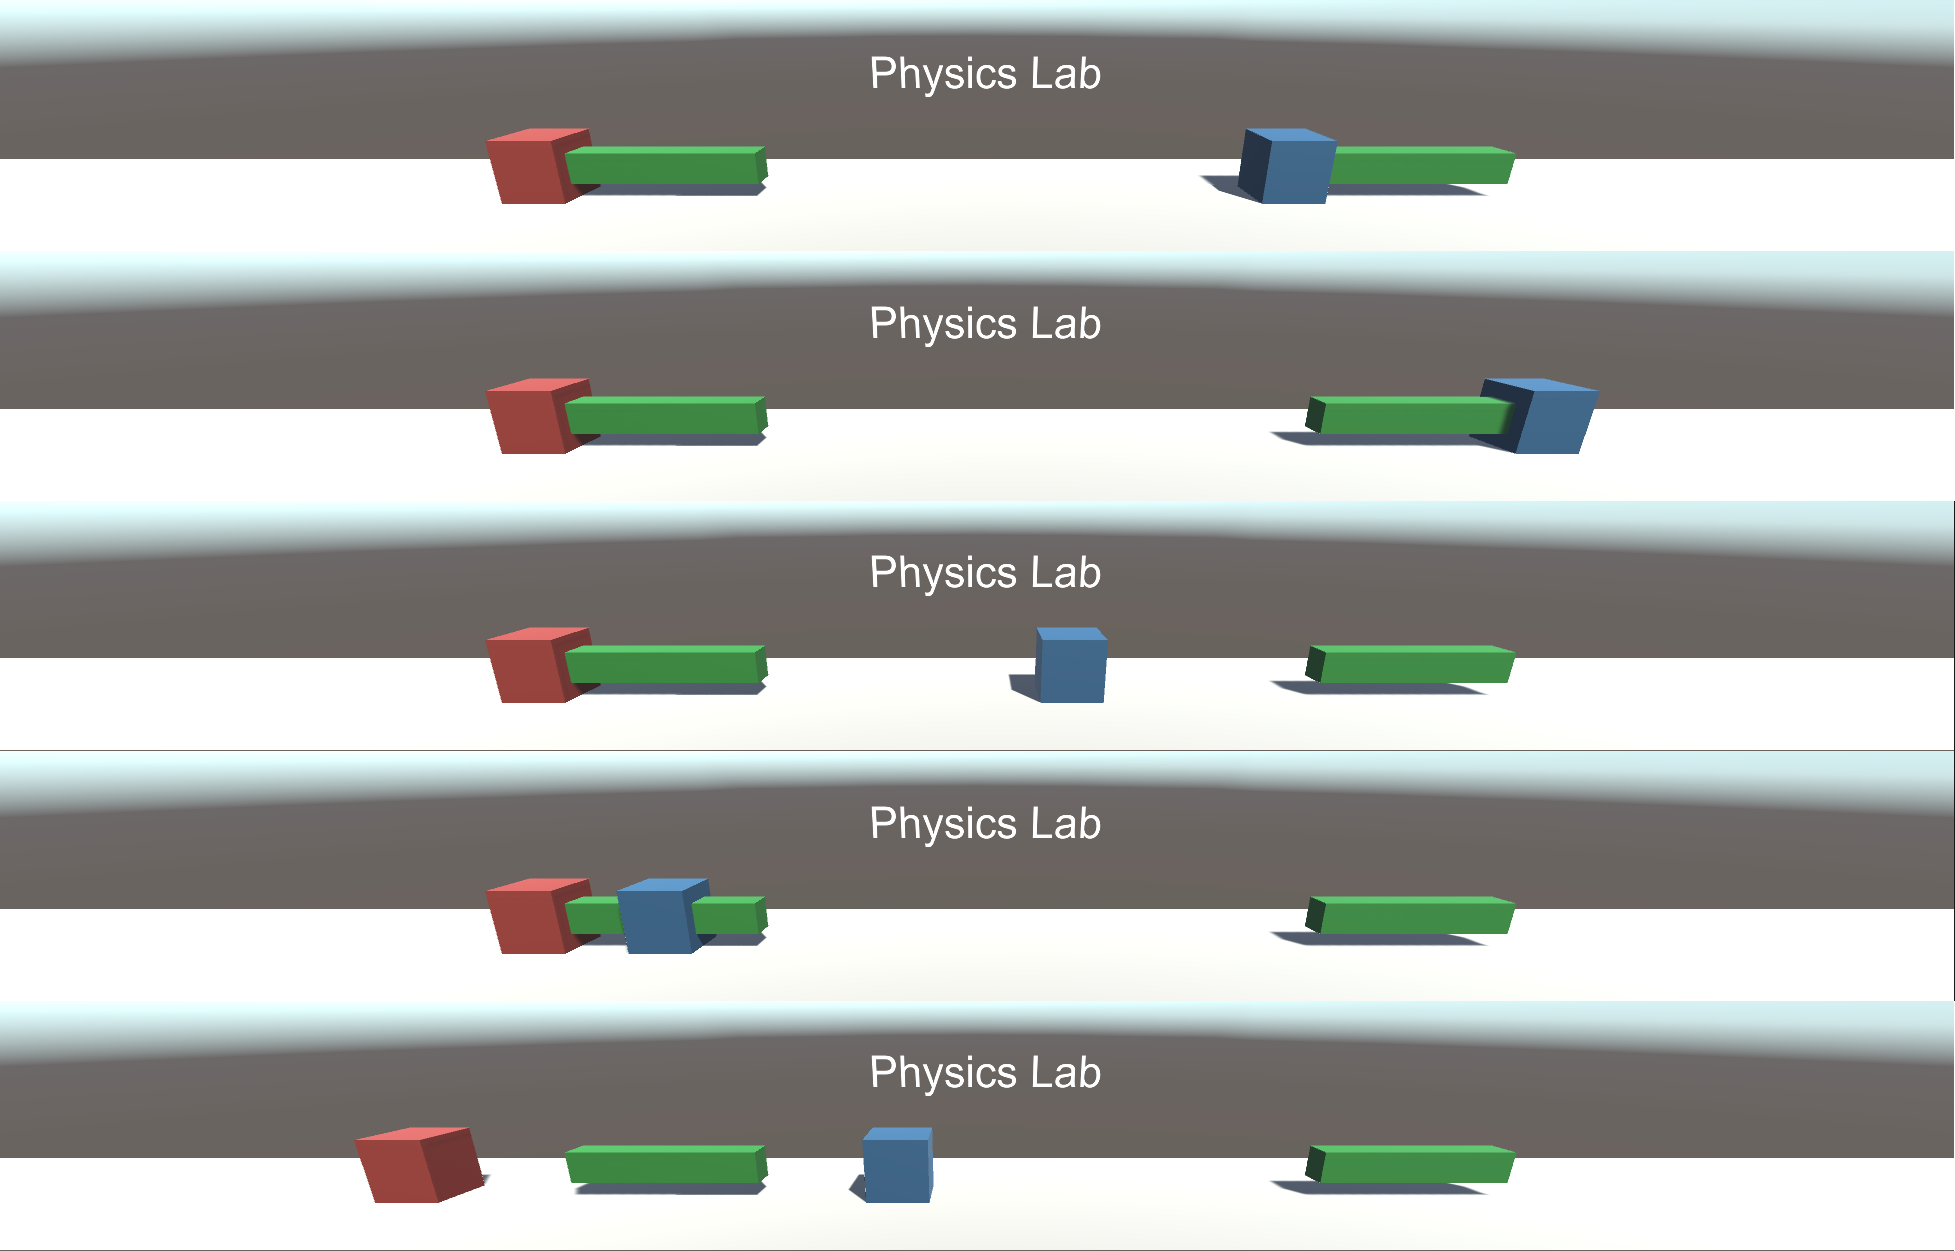
\includegraphics[width=0.9\linewidth]{assets/project_side_view_merged.png}
\scriptsize
\caption{Verschiedene Schritte vom Experiment}
\label{fig:project_side_view_merged}
\end{figure}
\noindent
Der blaue Würfel wird durch die rechte grüne Feder in Schwung gebracht. Er wird durch eine Windkonstante beschleunigt, bis er mit der zweiten linken Feder zusammenstösst. Der Zusammenstoss mit der Feder bewirkt, dass sich der rote Würfel und der blaue Würfel voneinander entfernen.

\newpage
\subsection{Teil 3: Inelastischer Stoss und Rotationsimpuls}

Die nachfolgender Auflistung bezieht sich auf Figure \ref{fig:duck}. Im ganzen Experiment wird die Reibungskraft vernachlässigt.
\begin{enumerate}
    \item Würfel 1 wird rückwärts gestossen und gleitet reibungsfrei – wir überlassen ihn seinem Schicksal.
    \item Würfel 2 fährt geradeaus weiter und stösst inelastisch mit einem L-förmigen Gebilde aus drei Würfeln zusammen.
    \item Bei Zusammenstoss heftet sich der Würfel 2 an das L-förmige Gegbilde an, sodass ein S-förmiges Gebilde entsteht.
    \item Das S-förmige Gebilde gleitet dank des inelastischen Stosses weiter und rotiert dabei.
\end{enumerate}

\begin{figure}[H] 
\centering\includegraphics[width=0.5\linewidth]{assets/duck.jpg}
\scriptsize
\caption{Duck}
\label{fig:duck}
\end{figure}
\noindent
Der Würfel 2 ist der Auslöser von Teil 3. Er stosst inelastisch auf ein neues Gebilde und heftet sich an. Dabei wirken Rotationsimpulse auf dem neuen Gebilde. Der Würfel 1 werden wir nicht weiter beachten.

\newpage
\section{Physikalische Beschreibung der einzelnen Vorgänge}
\subsection{Teil 2}
Dieses Teil des Experiments untersucht die Bewegung von zwei Würfeln und deren Stösse. Es gliedert sich in fünf physikalische Teilbewegungen:

\begin{enumerate}
    \item Würfel 1 oszilliert (Federkraft von Feder 1 wirkt auf Würfel 1)
    \item Würfel 1 wird durch eine Windkonstante angestossen
    \item Erste Stossphase vom Elastischen Stoss (Würfel 1 trifft auf Feder 2)
    \item Zweite Sossphase vom Elastischen Stoss (Impuls der gespeicherte Energie der Knautschzone fliesst)

\end{enumerate}
     In den Teilbewegungen 1–4 gleiten die Würfel reibungslos auf der Oberfläche.

\subsubsection{Oszillieren von Würfel 1}
Der Würfel 1 (blauer Würfel) wird durche eine Feder ins oszillieren gebracht. Zu Beginn wird der Würfel durch die bereits gespannte Feder in die gegengesetzte Richtung des zweiten Würfels (roter Würfel) beschleunigt. Sobald sich die Feder in der Ruhelage befindet, wird der Würfel 1 durch die Federkraft in die Richtung des Würfel 2 beschleunigt. Nachdem der Würfel die Position der Feder wieder erreicht, wird die Feder entfernt.
\newline
Die Federkraft kann wiefolgt berechnet werden:
\begin{equation}\label{eq:springforce}
    F =  k_{\text{Feder}} * \Delta l
\end{equation}

\scriptsize
\textbf{Equation (\ref{eq:springforce}):} $F$ Kraft in Newton [$N$], $k_{\text{Feder}}$ Federkonstatnte [$\frac{N}{m}$], $\Delta l$ Länge der Feder [$m$].
\normalsize
\medskip
\newline
Wobei die Änderung der Federlänge $\Delta l$ wiefolgt definiert ist:
\begin{equation}\label{eq:deltaL}
    \Delta l = l - l_0
\end{equation}

\scriptsize\textbf{Equation (\ref{eq:deltaL}):} $\Delta l$  Änderung der Federlänge [$m$], $l$ aktuelle Position [$m$], $l_0$ Startposition der Felder [$m$].
\newline
\normalsize
\medskip

\subsubsection{Windkonstante}
Der Würfel 1 (blauer Würfel) wird durch eine Windkraft beschleunigt, bis er die Feder des zweiten Würfels (roter Würfel) berührt.
Diese Windkraft wird durch eine konstante Krafteinwirkung auf den Würfel 1 umgesetzt.
\newline
Die Beschleunigung kann durch foglende Formel berechnet werden:
\begin{equation}\label{eq:constForce}
    F = m  a
\end{equation}

\scriptsize\textbf{Equation (\ref{eq:constForce}):} $F$ Kraft in Newton [$N$], $m$ Masse [$kg$], $a$ Beschleunigung 
[$\frac{m}{s^2}$].
\normalsize
\medskip

\subsubsection{Erste Stossphase vom Elastischen Stoss}
Zu Beginn der ersten Stossphase ist die Feder 2 in der Ruhelage. Der Würfel 1 (blauer Würfel) triff auf die Feder und verformt diese bis an den Kompressionspunkt. Dabei baut sich potentielle Energie in der Knautschzone auf.
Um diese Energie auszurechnen muss jedoch zuerst die kinetische Energie des Würfels berechnet werden.
\newline
Mit folgender Formel kann die kinetische Energie des Würfel 1 berechnet werden:
\begin{equation}\label{eq:kinEnerg}
E_{kin} = \frac{1}{2} mv^2
\end{equation}

\scriptsize
\textbf{Equation (\ref{eq:kinEnerg}):} $E_{kin}$ kinetische Energie des Würfels [$J$], $m$ Masse des Würfels [$kg$], $v$ Geschwindigkeit des Würfels [$\frac{m}{s}$].
\normalsize
\medskip
\newline
Anschliessend wird beim Aufprall die kinetische Energie des Würfels in potentielle Energie der Feder durch einen Impuls übertragen. Da die Geschwindigkeit des Würfel 2 0 beträgt, kann dieser Term weggelassen werden:
\begin{equation}\label{eq:impulsStoss1}
\vec{p_{in}} = m_{\text{Würfel1}} * \vec{v_{\text{Würfel1}}} + m_{\text{Würfel2}}
\end{equation}

\scriptsize
\textbf{Equation (\ref{eq:impulsStoss1}):} $\vec{p}$ Impuls-Vektor der in die Feder fliesst [$\text{kg} *\text{m/s}$], $m$ Masse des Würfels [$kg$], $\vec{v}$ Geschwindigkeits-Vektor des Würfels [$\frac{m}{s}$].
\normalsize
\medskip
\newline
Für Objekte, die elastisch verformbar sind (wie Federn), kann die potentielle Energie durch Hooke'sches Gesetz beschrieben werden:

\begin{equation}\label{eq:potEnerg}
E_{pot} = \frac{1}{2} *  k_{\text{Feder}} * x^2
\end{equation}

\scriptsize
\textbf{Equation (\ref{eq:potEnerg}):} $E_{pot}$ potentielle Energie in Feder [$J$], $k_{\text{Feder}}$ Federkonstante [$\frac{N}{m}$], $x$ Auslenkung der Feder [m].
\normalsize
\medskip

\subsubsection{Zweite Stossphase vom Elastischen Stoss}
Zu Beginn der zweiten Stossphase befindet sich die Feder im Kompressionspunkt. Der Impulserhaltungssatz besagt, dass der Gesamtimpuls eines abgeschlossenen Systems vor und nach einem Zusammenstoss gleich bleibt, daher stosst die Feder die beiden Objekte, mit der in der ersten Stossphase aufgebauten potentiellen Energie, durch einen Impuls auseinander:

\begin{equation}\label{eq:impulserh}
E_{pot} = m_{\text{Würfel1}} * (v_{\text{Würfel1}})^2 +  m_{\text{Würfel2}} * (v_{\text{Würfel2}})^2
\end{equation}

\scriptsize
\textbf{Equation (\ref{eq:impulserh}):} $E_{pot}$ potentielle Energie in Feder [$J$], $m$ Masse des Würfels [$kg$], $v$ Geschwindigkeit des Würfels [$\frac{m}{s}$].
\normalsize
\medskip
\newline
Bei der Berechnung der jeweiligen kinetischen Energie des Würfels muss die Ungleichverteilung der Massen der Würfel berücksichtigt werden. Der Würfel 2 (roter Würfel) hat die doppelte Masse des Würfel 1 (blauer Würfel).
\newline
Dazu kann folgende Formel benutzt werden:

\begin{equation}\label{eq:vDis1}
\begin{aligned}
E_{\text{kin Würfel1}} = \frac{m_{\text{Würfel1}}}{m_{\text{Würfel1}} + m_{\text{Würfel2}}} * E_{\text{pot}}
\end{aligned}
\end{equation}
und
\begin{equation}\label{eq:vDis2}
\begin{aligned}
E_{\text{kin Würfel2}} = \frac{m_{\text{Würfel2}}}{m_{\text{Würfel1}} + m_{\text{Würfel2}}} * E_{\text{pot}}
\end{aligned}
\end{equation}

\scriptsize
\textbf{Equation (\ref{eq:vDis1}) und (\ref{eq:vDis2}):} $E_{\text{kin Würfel}}$ Kinetische Energie der Würfel      [$J$], $m$ Masse des Würfels [$m$], $E_{pot}$ potentielle Energie in Feder [$J$].
\normalsize
\medskip
\newline
Dadruch lässt sich das Engergieerhaltungsgesetz darstellen:

\begin{equation}\label{eq:Energieerhalt}
E_{pot} = E_{\text{kin Würfel 1}} + E_{\text{kin Würfel 2}}
\end{equation}

\scriptsize
\textbf{Equation (\ref{eq:Energieerhalt}):} $E_{pot}$ Potentielle Energie in Feder [$J$], Kinetische Enerige in Würfel [$J$].
\normalsize
\medskip
\newline
Da es sich um einen elatsischen Stoss handelt, werden die Würfel voneinandern weggestossen.
\newline
Die jeweilige Krafteinwirkung auf den Würfel kann mitfolgender Formel berechnet werden:

\begin{equation}\label{eq:newtonCube}
F = \frac{m * v}{\Delta t}
\end{equation}

\scriptsize
\textbf{Equation (\ref{eq:newtonCube}):} $F$ Kraft in Newton [$N$], $m$ Masse [$kg$], $v$ Geschwindigkeit des Würfels [$\frac{m}{s}$], $\Delta t$ Zeit in Sekunden [$s$].
\normalsize
\medskip

\newpage

\subsection{Teil 3}
Dieses Teil des Experiments untersucht die Bewegung von einem Wüfel und einem L-förmigen Gebilde. Es gliedert sich in zwei physikalische Teilbewegungen:

\begin{enumerate}
    \item Würfel 2 stosst inelastisch auf L-förmiges Gebilde und haftet sich an
    \item Neues S-förmiges Gebilde fährt nach dem Stoss weiter und rotiert um den Schwerpunkt
\end{enumerate}
In den zwei Teilbewegungen gleiten die Würfel reibungslos auf der Oberfläche.
\subsubsection{Inelastischer Stoss von Würfel 2}
Der Würfel 2 gleitet nach dem elastischen Stoss weiter und stosst auf ein L-förmiges Gebilde und haftet sich an. Das L-förmige Gebilde besteht aus drei Würfel, welche alle gleich Schwer sind, wie Würfel 2. Somit bewegt sich das neu S-förmige Gebilde mit einer um 1/4 verringerter Geschwindigkeit weiter. Die gemeinsame Geschwindigkeit vom inelastischen Stoss kann mit folgender Formel berechnet werden:

\begin{equation}\label{eq:inelasticPush}
v_{gem} = \frac{p_{ges}}{m_{ges}} = \frac{m1*v1 + m2*v2}{m1 + m2}
\end{equation}

\scriptsize
\textbf{Equation (\ref{eq:inelasticPush}):} $v$ $\frac{m}{s}$, $m$ Masse [$kg$]
\subsubsection{Rotationsimpulse S-förmiges Gebilde}
\normalsize
\medskip
Um den Rotationsimpuls eines gleitenden und rotierenden Objektes zu berechnen verwenden wir zwei Formeln. Um den Drehimpuls eines gleitenden Körpers zu berechnen und zu beweisen, dass der Drehimpuls erhalten bleibt, wenn keine Schwerkraft angewendet wird, nutzen wir folgende Formeln:

\begin{equation}\label{eq:angularMomentumGlide}
L = R \times p
\end{equation}

\scriptsize
\textbf{Equation (\ref{eq:angularMomentumGlide}):} $L$ Drehimpuls $N$ * $m$ * $s$, $R$ Abstand der beiden Center $m$, $p$ Schwung $Ns$
\subsubsection{Rotationsimpulse S-förmiges Gebilde}
\normalsize
\medskip

\newpage

\section{Implementierung}
\subsection{Teil 2}
In diesem Abschnitt zeigen wir die Implementierung mit Screenshots der Simulation aus Unity.
\subsubsection{Oszillieren von Würfel 1}
\begin{figure}[H] 
\centering
\includegraphics[width=0.9\linewidth]{assets/StartingPosition_1.png}
\scriptsize
\caption{Oszillieren von Würfel 1}
\label{fig:StartingPosition_1}
\end{figure}
Die Anfangsposition vom Würfel 1 (blauer Würfel) wurde auf x = 5 festgelegt, die Masse beträgt m = 1 kg. Die Feder 1 hat ihren Mittelpunkt bei x = 7 und eine Federkonstante von 1 $N$. Die erforderliche Federkraft kann wie folgt berechnet werden:
\begin{subequations}\label{eq:oszillate}
    \begin{align}
    F =  k_{\text{Feder}} * \Delta l
    \end{align}
\end{subequations}

\scriptsize
\textbf{Equation (\ref{eq:oszillate}):} $F$ Kraft in Newton [$N$], $k_{\text{Feder}}$ Federkonstatnte [$\frac{N}{m}$], $\Delta l$ Länge der Feder [$m$].
\normalsize
\medskip
\newline
Die berechnete Kraft mit $k_{\text{Feder}}$ = 1 $N$ und \( \Delta \)l = -2 m ist somit F = -2.
\begin{figure}[H] 
\centering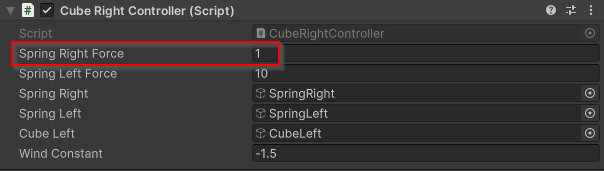
\includegraphics[width=0.9\linewidth]{assets/SpringRightForce.png}
\scriptsize
\caption{Federkonstante Feder 1}
\label{fig:SpringRightForce}
\end{figure}
\begin{figure}[H] 
\centering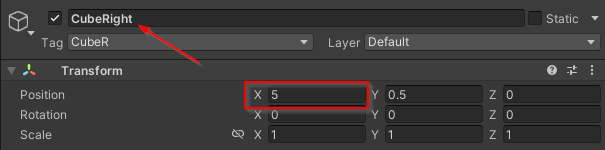
\includegraphics[width=0.9\linewidth]{assets/CubeRight_X.png}
\scriptsize
\caption{Anfangsposition Würfel 1}
\label{fig:CubeRight_X}
\end{figure}
\begin{figure}[H] 
\centering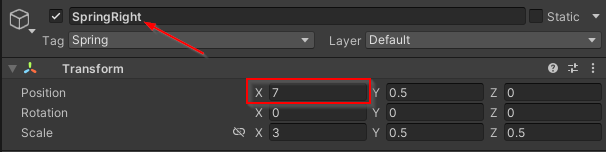
\includegraphics[width=0.9\linewidth]{assets/SpringRight_X.png}
\scriptsize
\caption{Anfangsposition Feder 1}
\label{fig:SpringRight_X}
\end{figure}

\subsubsection{Windkonstante}
\begin{figure}[H] 
\centering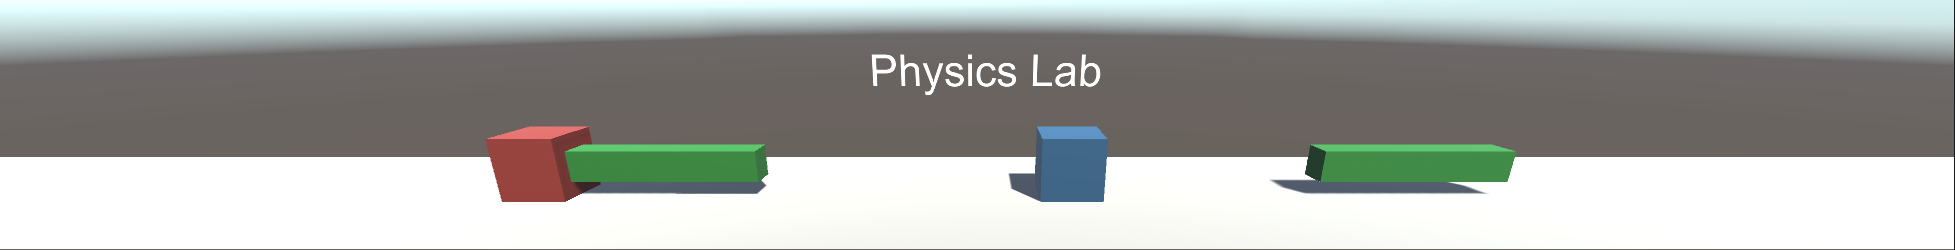
\includegraphics[width=0.9\linewidth]{assets/project_side_view_3.png}
\scriptsize
\caption{Windkonstante wird auf Würfel 1 angewendet}
\label{fig:project_side_view_3}
\end{figure}
Wir entfernen die Feder 1 vom Würfel, sodass dieser nicht mehr oszilliert. Gleichzeitig setzt ein Wind ein, der den
Würfel 1 beschleunigt. Der Würfel 1 hat eine Masse $m$ = 1 kg und die Windkonstante beträgt $F$ = -1.5 $N$. Der Würfel gleitet reibungsfrei.
Die Beschleunigung kann durch foglende Formel berechnet werden:
\begin{equation}\label{eq:constantForce}
    F = m  a
\end{equation}

\scriptsize
\textbf{Equation (\ref{eq:constantForce}):} $F$ Kraft in Newton [$N$], $m$ Masse [$kg$], $a$ Beschleunigung 
[$\frac{m}{s^2}$].
\normalsize
\medskip
\newline
Somit ist die Maximalbeschleunigung $a$ = -1.5 m/\( s^2 \).

\begin{figure}[H] 
\centering
\includegraphics[width=0.9\linewidth]{assets/cubeRight_mass.png}
\scriptsize
\caption{Masse vom Würfel 1}
\label{fig:cubeRight_mass}
\end{figure}

\begin{figure}[H] 
\centering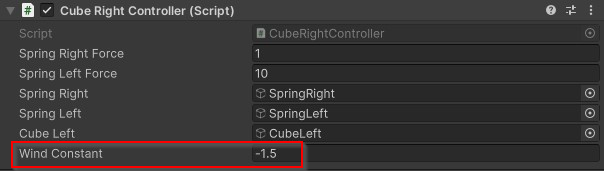
\includegraphics[width=0.9\linewidth]{assets/wind_constant.png}
\scriptsize
\caption{Windkonstante}
\label{fig:wind_constant}
\end{figure}
\newpage

\subsubsection{Erste Stossphase vom Elastischen Stoss}
\begin{figure}[H] 
\centering
\includegraphics[width=0.9\linewidth]{assets/project_side_view_4.png}
\scriptsize
\caption{Würfel 1 stosst auf Feder 2}
\label{fig:project_side_view_4}
\end{figure}
In dieser Phase wird Energie in der Knautschzone gespeichert. Durch integrieren der Beschleunigung vom Würfel 1 stosst dieser elastisch mit einer Maximalgeschwindigkeit von -5.929 m/s auf die Feder 2. Die Feder 2 hat eine Startposition von x = -7. Der Wind stoppt, sobald der Stoss beginnt.
Somit kann die kinetische Energie des Würfel 1 berechnet werden:
\begin{equation}\label{eq:kinEnergie}
E_{kin} = \frac{1}{2} mv^2
\end{equation}

\scriptsize
\textbf{Equation (\ref{eq:kinEnergie}):} $E_{kin}$ kinetische Energie des Würfels [$J$], $m$ Masse des Würfels [$kg$], $v$ Geschwindigkeit des Würfels [$\frac{m}{s}$].
\normalsize
\medskip
\newline
Somit haben wir eine kinetische Energie vom Würfel 1 von $E_{kin}$ = 17.578 $J$ beim Zusammenstoss mit der Feder.
\begin{figure}[H] 
\centering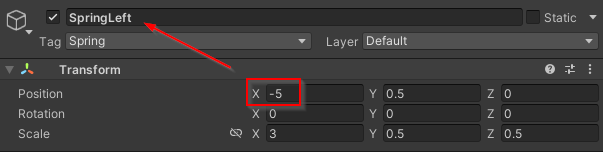
\includegraphics[width=0.9\linewidth]{assets/SpringLeft_X.png}
\scriptsize
\caption{Position Feder 2}
\label{fig:SpringLeft_X}
\end{figure}

\noindent
Die Federkonstante beträgt 10 $N/m$ und die ausgedehnte Auslennkung beträgt x = 3 m. Für die Feder 1 kann die potentielle Energie durch Hooke'sches Gesetz berechnet werden:

\begin{equation}\label{eq:potEnergy}
E_{pot} = \frac{1}{2} *  k_{\text{Feder}} * x^2
\end{equation}

\scriptsize
\textbf{Equation (\ref{eq:potEnergy}):} $E_{pot}$ potentielle Energie in Feder [$J$], $k_{\text{Feder}}$ Federkonstante [$\frac{N}{m}$], $x$ Auslenkung der Feder [$m$].
\normalsize
\medskip
\newline
Damit können wir die maximale Energie berechnen, welche die Feder 2 aufnehmen kann. Wir können mit der kinetischen Energie vom Würfel 1 auch die Auslenkung der Feder berechnen.Angenommen die Feder 2 würdekomplett zusammengedrückt, so ergäb das eine maximale potentielle Energie von $Epot$ = 45 $J$.
Mit der vorherigen Berechnung stösst der Würfel 1 mit $E_{kin}$ = 17.578 $J$ auf die Feder, somit wird die Feder um a = 1.874 $m$ gestaucht.

\begin{figure}[H] 
\centering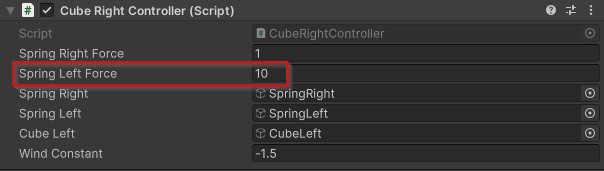
\includegraphics[width=0.9\linewidth]{assets/SpringLeftForce.png}
\scriptsize
\caption{Federkonstante Feder 2}
\label{fig:SpringLeftForce}
\end{figure}
\normalsize
\medskip
\noindent

\subsubsection{Zweite Stossphase vom Elastischen Stoss}
\begin{figure}[H] 
\centering
\includegraphics[width=0.9\linewidth]{assets/project_side_view_5.png}
\scriptsize
\caption{Energie fliesst als Impuls auf beide Würfel}
\label{fig:project_side_view_5}
\end{figure}
In der zweiten Stossphase sorgt die gespeicherte potentielle Energie dafür, dass noch einmal so viel Impuls fliesst, wie in der ersten Stossphase geflossen ist. Der Würfel 1 wirkt mit einer Energie von $E_{kin}$ = 17.578 $J$ und der Würfel 2 mit $E_{kin}$ = 0 $J$, da dieser sich nicht bewegt. Die aufzuteilende potentielle Energie ergibt sich aus folgender Gleichung:
\begin{equation}\label{eq:impulserhalt}
E_{pot} = m_{\text{Würfel1}} * (v_{\text{Würfel1}})^2 +  m_{\text{Würfel2}} * (v_{\text{Würfel2}})^2
\end{equation}

\scriptsize
\textbf{Equation (\ref{eq:impulserhalt}):} $E_{pot}$ potentielle Energie in Feder [$J$], $m$ Masse des Würfels [$kg$], $v$ Geschwindigkeit des Würfels [$\frac{m}{s}$].
\newline

\normalsize
\noindent
Also erhalten wir eine potentielle Energie von $E_{kin}$ = 17.578 $J$, welche wir nun auf die beiden Würfel aufteilen müssen. Dafür verwenden wir folgende Formel:

\begin{equation}\label{eq:vDist1}
\begin{aligned}
E_{\text{kin Würfel1}} = \frac{m_{\text{Würfel1}}}{m_{\text{Würfel1}} + m_{\text{Würfel2}}} * E_{\text{pot}}
\end{aligned}
\end{equation}
und
\begin{equation}\label{eq:vDist2}
\begin{aligned}
E_{\text{kin Würfel2}} = \frac{m_{\text{Würfel2}}}{m_{\text{Würfel1}} + m_{\text{Würfel2}}} * E_{\text{pot}}
\end{aligned}
\end{equation}

\scriptsize
\textbf{Equation (\ref{eq:vDist1}) und (\ref{eq:vDist2}):} $E_{\text{kin Würfel}}$ Kinetische Energie des Würfels [$J$], $m$ Masse des Würfels [$m$], $E_{\text{pot}}$ potentielle Energie Feder [$J$].
\newline

\normalsize
\noindent
Somit erhaltet Würfel 1 $E_{kin}$ = 5.859 $J$ und Würfel 2 $E_{kin}$ = 11.718 $J$ als Impuls in der zweiten Stossphase.

\newpage
\subsection{Teil 3}
\subsubsection{TBD}

\newpage
\section{Resultat}
Die Figure \ref{fig:velocity_comparison} veranschaulicht die Geschwindigkeit der Würfel in den drei Phasen von Teil 2. Der Würfel 1 oszilliert zwischen x = 2 und x = -2 bis wir die Feder entfernen. Danach wirkt die Windkonstante. Ersichtlich im Zeitintervall von 3 s bis ca. 7.5 s. Die dritte Phase beeinträchtigt beide Würfel. Sie werden mit einer konstanten Geschiwindigkeit voneinander weggestosst. Die beiden Würfel gleiten danach ohne Reibung.

\vspace{-1em} % Adjust the value as needed to reduce the gap
\begin{figure}[H] 
\centering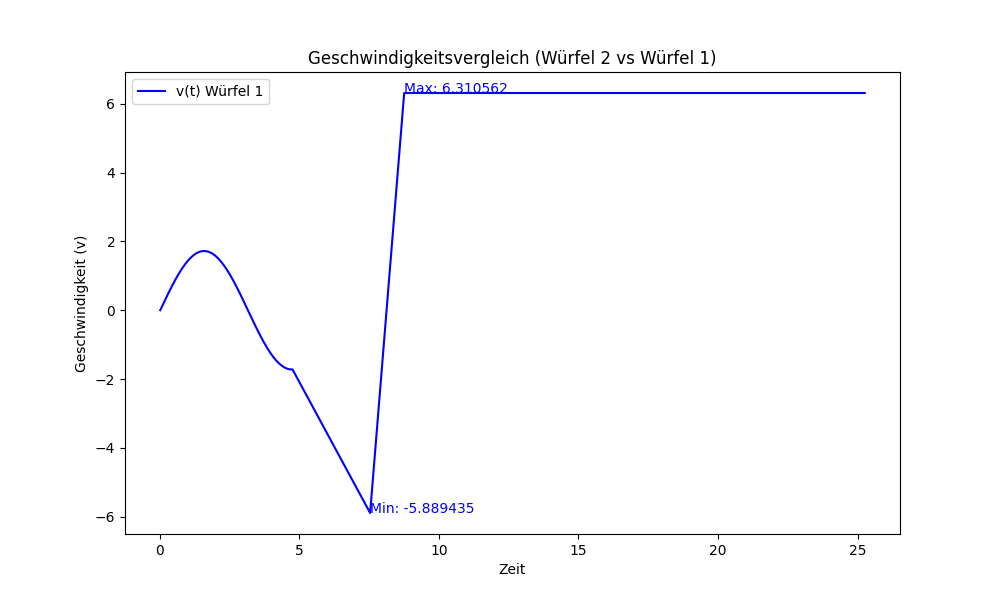
\includegraphics[width=0.75\linewidth]{assets/velocity_comparison.png}
\scriptsize
\caption{Geschwindigkeitsdiagramm der beiden Würfel}
\label{fig:velocity_comparison}
\end{figure}
\noindent
Die Position der Würfel wird in der Figure \ref{fig:position_comparison} veranschaulicht. Der Würfel 1 oszilliert von der Feder 1 bis wir die Feder entfernen und die Windkonstante greifft. Danach wird bis zum Zusammenstoss die Position vom Würfel 1 immer kleiner. Beim Zusammenstoss gehen die beiden Würfel auseinander.

\vspace{-1em} % Adjust the value as needed to reduce the gap
\begin{figure}[H] 
\centering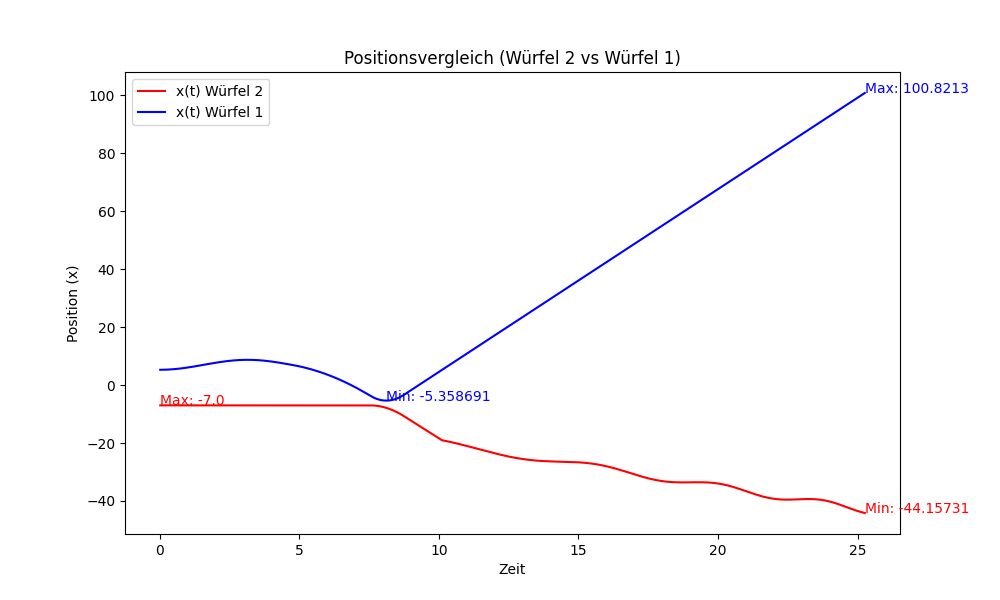
\includegraphics[width=0.75\linewidth]{assets/position_comparison.png}
\scriptsize
\caption{Positionsvergleich der beiden Würfel}
\label{fig:position_comparison}
\end{figure}

\noindent
Die Figure \ref{fig:force_comparison} veranschaulicht die Kraft der Würfel in den drei Phasen der Aufgabe. Die Kraft vom Würfel 1 oszilliert bis wir die Feder entfernen. Die Windkraft wirkt direkt und konstant auf den Würfel 1. Bis da hin wirkt keine Kraft auf den Würfel 2. Beim Zusammenstoss wirkt eine Kraft auf beide Würfel.
\begin{figure}[H] 
\centering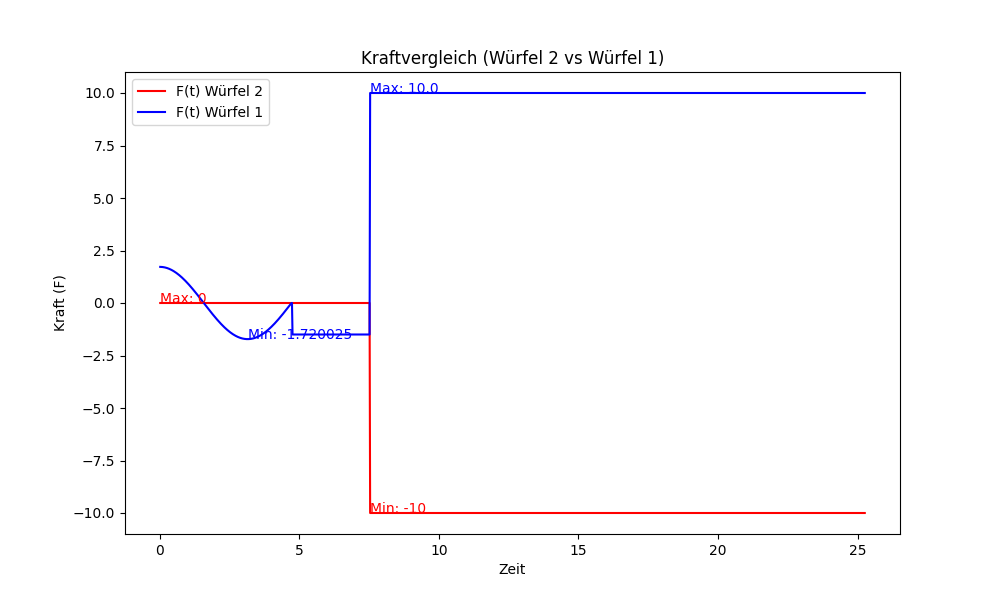
\includegraphics[width=0.75\linewidth]{assets/force_comparison.png}
\scriptsize
\caption{Kräftevergleich der beiden Würfel}
\label{fig:force_comparison}
\end{figure}

\newpage

\section{Rückblick}
TBD
\newpage

\listoffigures
\clearpage
\normalsize

\newpage

\section{Appendix}
\listoflistings
\normalsize

\clearpage
\appendix

\section{Source codes}
\begin{lstlisting}[caption={CubeRightController.cs}, label={CubeRightController}, basicstyle=\ttfamily\small]
using System.Collections;
using System.Collections.Generic;
using UnityEngine;

using System.IO;
using UnityEditor;
using UnityEngine.SceneManagement;
using System;
using UnityEngine.Assertions.Must;

/*
    Accelerates the cube to which it is attached, modelling an harmonic oscillator.
    Writes the position, velocity and acceleration of the cube to a CSV file.
    
    Remark: For use in "Physics Engines" module at ZHAW, part of physics lab
    Author: kemf
    Version: 1.0
*/
public class CubeRightController : MonoBehaviour
{
    private Rigidbody rigidBody;

    public int springRightForce;
    public int springLeftForce;
    public GameObject springRight;
    public GameObject springLeft;
    public GameObject cubeLeft;
    public float windConstant;
    public bool oscillate;


    private float currentTimeStep;
    private List<List<float>> timeSeries;
    private Phase phase = Phase.oscillator;
    private float cubeRightForceX;
    private float cubeLeftForceX;
    private float springLeftFurthestPointRight;

    enum Phase
    { oscillator, wind, collision, none }

    // Start is called before the first frame update
    void Start()
    {
        rigidBody = GetComponent<Rigidbody>();
        timeSeries = new List<List<float>>();
        timeSeries = new List<List<float>>();
        springLeftFurthestPointRight = springLeft.transform.position.x + GetSpringLeftWidth() / 2f;
    }

    // FixedUpdate can be called multiple times per frame
    void FixedUpdate()
    {
        currentTimeStep += Time.deltaTime;
        switch(phase)
        {
            case Phase.oscillator:
                var deltaL = rigidBody.position.x - springRight.transform.position.x;
                cubeRightForceX = -deltaL * springRightForce;
                
                AddForceToRigidBody(cubeRightForceX);

                //Cube comes back from spring and now only the wind carries the cube
                if (rigidBody.position.x < springRight.transform.position.x && rigidBody.velocity.x < 0 && !oscillate) {
                    cubeRightForceX = 0;
                    phase = Phase.wind;
                }

                break;

            case Phase.wind:
                cubeRightForceX = windConstant;
                AddForceToRigidBody(cubeRightForceX);

                if(rigidBody.position.x <= springLeftFurthestPointRight)
                {
                    phase = Phase.collision;
                }

                break;

            case Phase.collision:
                cubeRightForceX = springLeftForce;
                AddForceToRigidBody(cubeRightForceX);

                cubeLeftForceX = -cubeRightForceX;
                cubeLeft.GetComponent<Rigidbody>().AddForce(new Vector3(cubeLeftForceX, 0f, 0f));

                if (rigidBody.position.x >= springLeftFurthestPointRight)
                {
                    phase = Phase.none;
                }
                break;

            case Phase.none:
                if (rigidBody.position.x >= 15) {
                    UnityEditor.EditorApplication.isPlaying = false;
                }
                break;

        }
        timeSeries.Add(new List<float>() { currentTimeStep, cubeLeft.GetComponent<Rigidbody>().position.x, cubeLeft.GetComponent<Rigidbody>().velocity.x, cubeLeftForceX, rigidBody.position.x, rigidBody.velocity.x, cubeRightForceX });
    }

    private void AddForceToRigidBody(float cubeRightForceX) {
        rigidBody.AddForce(new Vector3(cubeRightForceX, 0f, 0f));
    }

    // Helper function to get the width of springLeft
    private float GetSpringLeftWidth()
    {
        Renderer renderer = springLeft.GetComponent<Renderer>();
        if (renderer != null)
        {
            return renderer.bounds.size.x;
        }
        else
        {
            Debug.LogError("Renderer component not found on the object.");
            return 0f;
        }
    }

    void OnApplicationQuit() {
        WriteTimeSeriesToCSV();
    }

    void WriteTimeSeriesToCSV() {
        using (var streamWriter = new StreamWriter("data.csv")) {
            streamWriter.WriteLine("t,x(t) cubeL,v(t) cubeL,F(t) cubeL,x(t) cubeR,v(t) cubeR,F(t) cubeR");
            
            foreach (List<float> timeStep in timeSeries) {
                streamWriter.WriteLine(string.Join(",", timeStep));
                streamWriter.Flush();
            }
        }
    }
}
\end{lstlisting}
\newpage
\begin{lstlisting}[caption={Plotter.py}, label={Plotter}, basicstyle=\ttfamily\small]
import pandas as pd
import matplotlib.pyplot as plt

# Read the CSV file
df = pd.read_csv('../data.csv')

# Extract data from columns
t = df['t']
x_left = df['x(t) cubeL']
v_left = df['v(t) cubeL']
F_left = df['F(t) cubeL']
x_right = df['x(t) cubeR']
v_right = df['v(t) cubeR']
F_right = df['F(t) cubeR']

# Calculate min and max points
x_left_min, x_left_max = min(x_left), max(x_left)
v_left_min, v_left_max = min(v_left), max(v_left)
F_left_min, F_left_max = min(F_left), max(F_left)
x_right_min, x_right_max = min(x_right), max(x_right)
v_right_min, v_right_max = min(v_right), max(v_right)
F_right_min, F_right_max = min(F_right), max(F_right)

# Plotting x(t)
plt.figure(figsize=(10, 6))

plt.plot(t, x_left, label='x(t) Würfel 2', color='red')
plt.plot(t, x_right, label='x(t) Würfel 1', color='blue')

plt.xlabel('Zeit')
plt.ylabel('Position (x)')
plt.title('Positionsvergleich (Würfel 2 vs Würfel 1)')
plt.legend()

plt.text(t.iloc[x_left.idxmin()], x_left_min, f'Min: {x_left_min}', color='red')
plt.text(t.iloc[x_left.idxmax()], x_left_max, f'Max: {x_left_max}', color='red')
plt.text(t.iloc[x_right.idxmin()], x_right_min, f'Min: {x_right_min}', color='blue')
plt.text(t.iloc[x_right.idxmax()], x_right_max, f'Max: {x_right_max}', color='blue')

plt.savefig('position_comparison.png')
plt.close()

# Plotting v(t)
plt.figure(figsize=(10, 6))

plt.plot(t, v_left, label='v(t) Würfel 2', color='red')
plt.plot(t, v_right, label='v(t) Würfel 1', color='blue')

plt.xlabel('Zeit')
plt.ylabel('Geschwindigkeit (v)')
plt.title('Geschwindigkeitsvergleich (Würfel 2 vs Würfel 1)')
plt.legend()

plt.text(t.iloc[v_left.idxmin()], v_left_min, f'Min: {v_left_min}', color='red')
plt.text(t.iloc[v_left.idxmax()], v_left_max, f'Max: {v_left_max}', color='red')
plt.text(t.iloc[v_right.idxmin()], v_right_min, f'Min: {v_right_min}', color='blue')
plt.text(t.iloc[v_right.idxmax()], v_right_max, f'Max: {v_right_max}', color='blue')

plt.savefig('velocity_comparison.png')
plt.close()

# Plotting F(t)
plt.figure(figsize=(10, 6))

plt.plot(t, F_left, label='F(t) Würfel 2', color='red')
plt.plot(t, F_right, label='F(t) Würfel 1', color='blue')

plt.xlabel('Zeit')
plt.ylabel('Kraft (F)')
plt.title('Kraftvergleich (Würfel 2 vs Würfel 1)')
plt.legend()

plt.text(t.iloc[F_left.idxmin()], F_left_min, f'Min: {F_left_min}', color='red')
plt.text(t.iloc[F_left.idxmax()], F_left_max, f'Max: {F_left_max}', color='red')
plt.text(t.iloc[F_right.idxmin()], F_right_min, f'Min: {F_right_min}', color='blue')
plt.text(t.iloc[F_right.idxmax()], F_right_max, f'Max: {F_right_max}', color='blue')

plt.savefig('force_comparison.png')
plt.close()

\end{lstlisting}

\end{document}